\documentclass[11pt,letterpaper]{article}

\usepackage[margin=1in]{geometry}
\usepackage{graphicx}
\usepackage{tabularx}
\usepackage{array}
\usepackage{booktabs}
\usepackage{float}
\usepackage{ragged2e}
\usepackage[table]{xcolor}
\usepackage{enumitem}
\usepackage{amsmath,amssymb}
\usepackage{hyperref}
\usepackage{fancyhdr}

\hypersetup{colorlinks=true, linkcolor=black, urlcolor=blue, citecolor=black}

\setlength{\headheight}{14pt}
\pagestyle{fancy}
\fancyhf{}
\rhead{\thepage}
\lhead{\textit{PCBA System --- Project Report}}
\renewcommand{\headrulewidth}{0.4pt}

\newcolumntype{Y}{>{\RaggedRight\arraybackslash}X}

\title{\textbf{ECE404 Final Presentation Report} \\
       \large Consumer-Scale PCB Pick-and-Place / Reflow System}
\author{Group 3 \\
        Ainaan Qureshi \\
        Amara Coleman \\
        Andy Brinker \\
        Chuck O'Neill \\
      }
\date{\today}

\begin{document}

\maketitle
\newpage

\tableofcontents
\newpage

\section{Needs and Objectives}

\subsection{Needs} 
	While the distribution of information and the consistent growth in access to technology have made the feasibility and demand for rapid prototyping/consumer-aimed PCBA tools, the market for such tools is yet to be clearly defined. PCBA tools have typically been relegated to industrial use. In a commercial setting, testing physical components as opposed to simulating such components brings the benefit of not needing to model non-idealities. In a consumer setting, small-batch runs of PCBs may be unreasonable to produce due to cost. The expansion of small-scale PCBA tools can provide new avenues to both commercial and at-home users. 

\subsection{Objective}
	We aim to create a system which handles portions of the PCB manufacturing process. This machine should be affordable, precise enough to handle typical IC packages such as LQFP, and easy to maintain. The assembly of a PCB entails placing solder on the pads of an unpopulated board, placing components on their respective pads, and reflowing the solder in order to finish the process. A system to handle this process must manage the input of board information, solder paste, various ICs and board components, and the board itself in order to provide a finished assembled board. 

\section{Market Research and Comparison}
% comparison_table.tex
% Comparison: Voltera V-One vs. BotFactory SV2 vs. Proposed Design
% Requires in preamble:
%   \usepackage{tabularx}
%   \usepackage{array}
%   \usepackage{booktabs}
%   \usepackage{float}
%   \usepackage{ragged2e}
%   \usepackage[table]{xcolor}

\newcolumntype{Y}{>{\RaggedRight\arraybackslash}X}

\begin{table}[H]
\centering
\caption{Comparison of existing PCBA solutions and the proposed design.}
\label{tab:comparison}
\renewcommand{\arraystretch}{1.3}
\small
\begin{tabularx}{\textwidth}{|>{\bfseries}l|Y|Y|Y|}
\hline
\rowcolor{gray!15}
Specification & \textbf{Voltera V-One} & \textbf{BotFactory SV2} & \textbf{Proposed Design} \\ \hline
Price                    & \$3{,}499 & \$19{,}999 & --- \\ \hline
Capabilities             & Conductive ink trace printing; solder paste dispensing; drilling (vias); on-board reflow
                         & Conductive ink trace printing; solder paste dispensing; component placement; on-board reflow
                         & Solder paste dispensing; component placement; on-board reflow \\ \hline
Min.\ Mechanical Feature & 0.1\,mm & 0.1\,mm & 0.2\,mm \\ \hline
Layer Capacity           & 2 & 2 & 1 \\ \hline
Print / Build Area       & 8.7\,in $\times$ 11.8\,in & 4.6\,in $\times$ 5.5\,in & 4\,in $\times$ 6\,in \\ \hline
\end{tabularx}
\end{table}


\section{Objective Tree}

\begin{figure}[H]
\centering
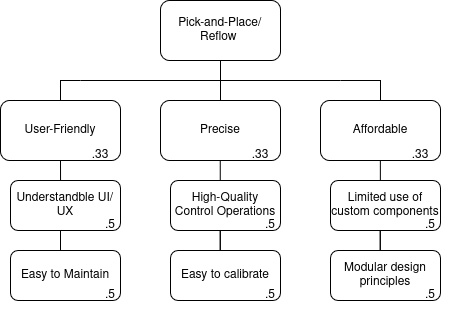
\includegraphics[width=0.85\textwidth]{objective_tree.png}
\caption{Objective tree for the proposed pick-and-place / reflow system.}
\label{fig:objtree}
\end{figure}

\section{Requirements Specification}

\subsection{Marketing Requirements}
% Add your marketing requirements here.
\begin{enumerate}
    \item The system must be easy to use
    \item The system should have a touchscreen gui
\end{enumerate}

\subsection{Engineering Requirements}
\begin{enumerate}
    \item The device must handle centroid files from Kicad and Altium.
    \item The device must be capable of precision defined by LQFP packages.
    \item The device must handle power motors, logic, and reflow heat separately.
    \item The device must receive power from standard 120VAC wall outlet.
    \item The device must have a simple GUI user interface.
    \item The device must have mechanical safety features incorporating limit switches (or comparable) on all axes of linear movement.
    \item The device must have thermal safety features which cut power to the system in the case of failure.
    \item Device must comply with safety standards for consumer electronics involving mains power.
\end{enumerate}



\section{Engineering Standards}

\begin{table}[H]
\centering
\caption{Standards}
\label{tab:standards}
\renewcommand{\arraystretch}{1.3}
\small
\begin{tabularx}{\textwidth}{|>{\bfseries}l|l|Y|}
\hline
\rowcolor{gray!15}
Standard & \textbf{Version} & \textbf{Description} \\ \hline
UL 499              & 13th ed., 2014 (with revisions) & Electric heating appliances. Covers thermal cutoffs, fault behavior, and overtemperature protection. \\ \hline
ANSI/RIA R15.06     & 2012                            & Reference for safety standards in industrial robotics systems: limit-switch and safe-state concepts. \\ \hline
IPC-2581            & Rev.\ C, 2022                   & Reference for centroid file standards. \\ \hline
UL 61010-1          & Ed.\ 3, 2012 (rev.\ through 2024) & Safety requirements for electrical equipment for measurement, control, and laboratory use. \\ \hline
\end{tabularx}
\end{table}



\section{Functional Decomposition}

\subsection{Level 0 --- System Overview}
\begin{figure}[H]
\centering
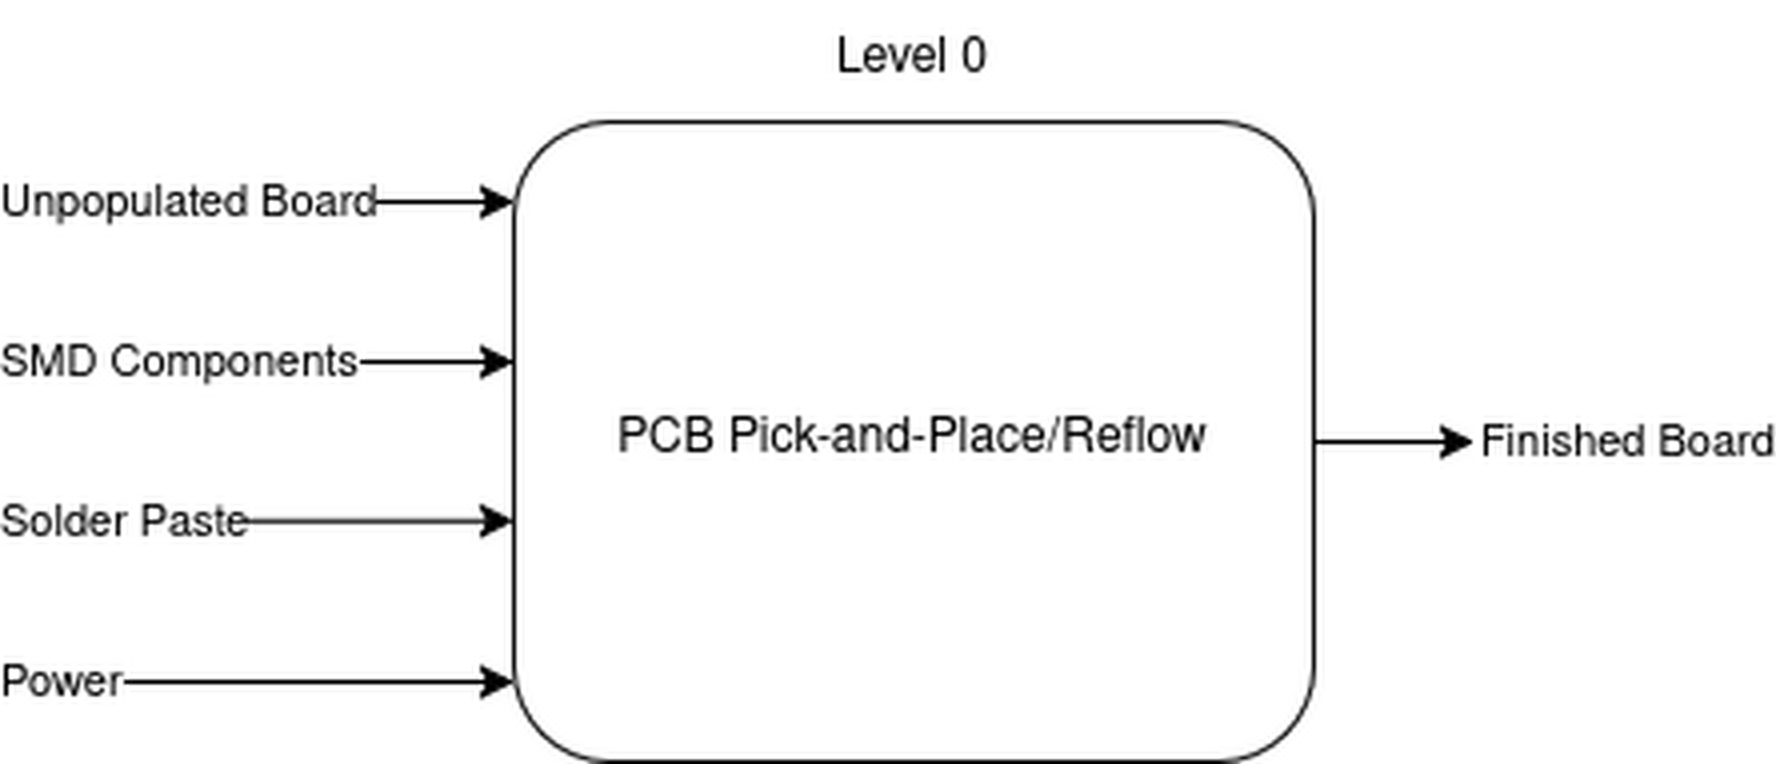
\includegraphics[width=0.7\textwidth]{Level0.png}
\caption{Level 0 Decompositon}
\label{fig:level0}
\end{figure}

\subsection{Level 1 Decomposition}
\begin{figure}[H]
\centering
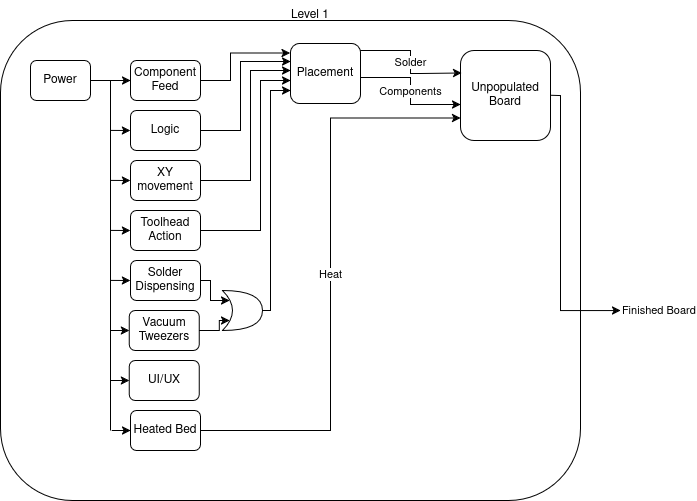
\includegraphics[width=\textwidth]{Level_1.png}
\caption{Level 1 Decomposition}
\label{fig:level1}
\end{figure}

\subsection{Level 2 --- Power}
\begin{figure}[H]
\centering
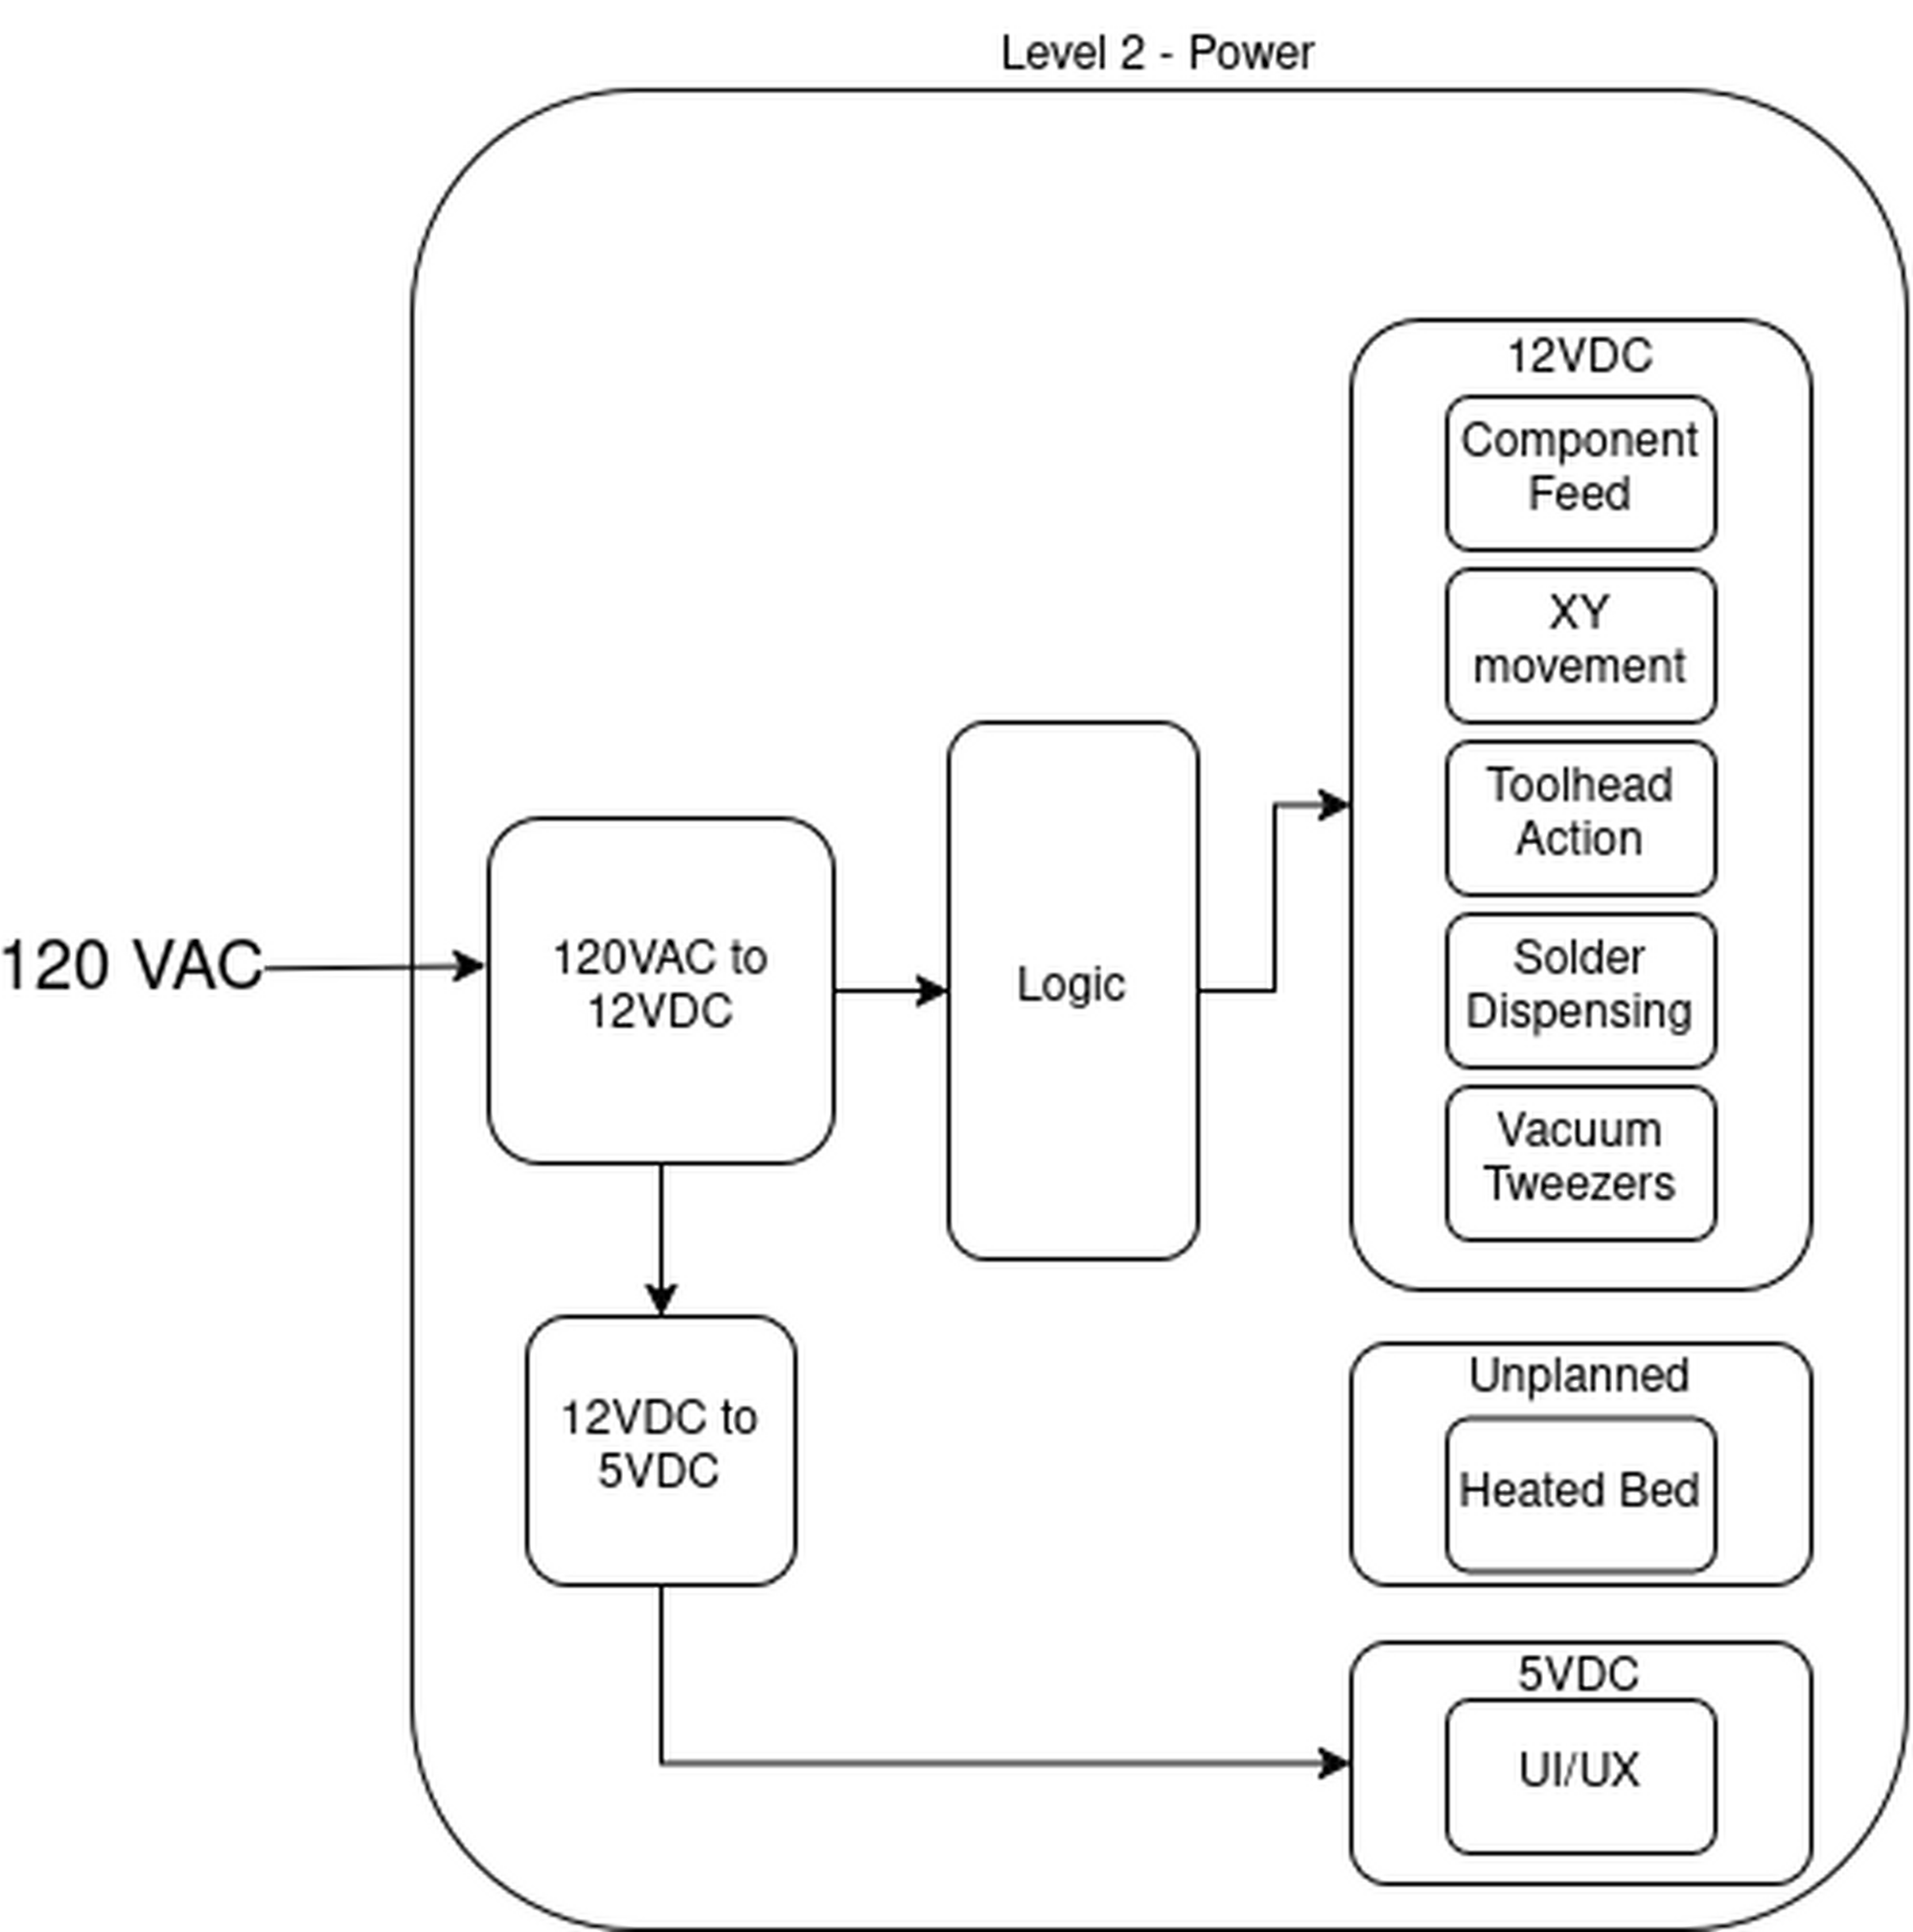
\includegraphics[width=0.85\textwidth]{Level2_power.png}
\caption{Level 2 Decomposition - Power}
\label{fig:level2_power}
\end{figure}

\subsection{Level 2 --- Logic \& UI/UX}
\begin{figure}[H]
\centering
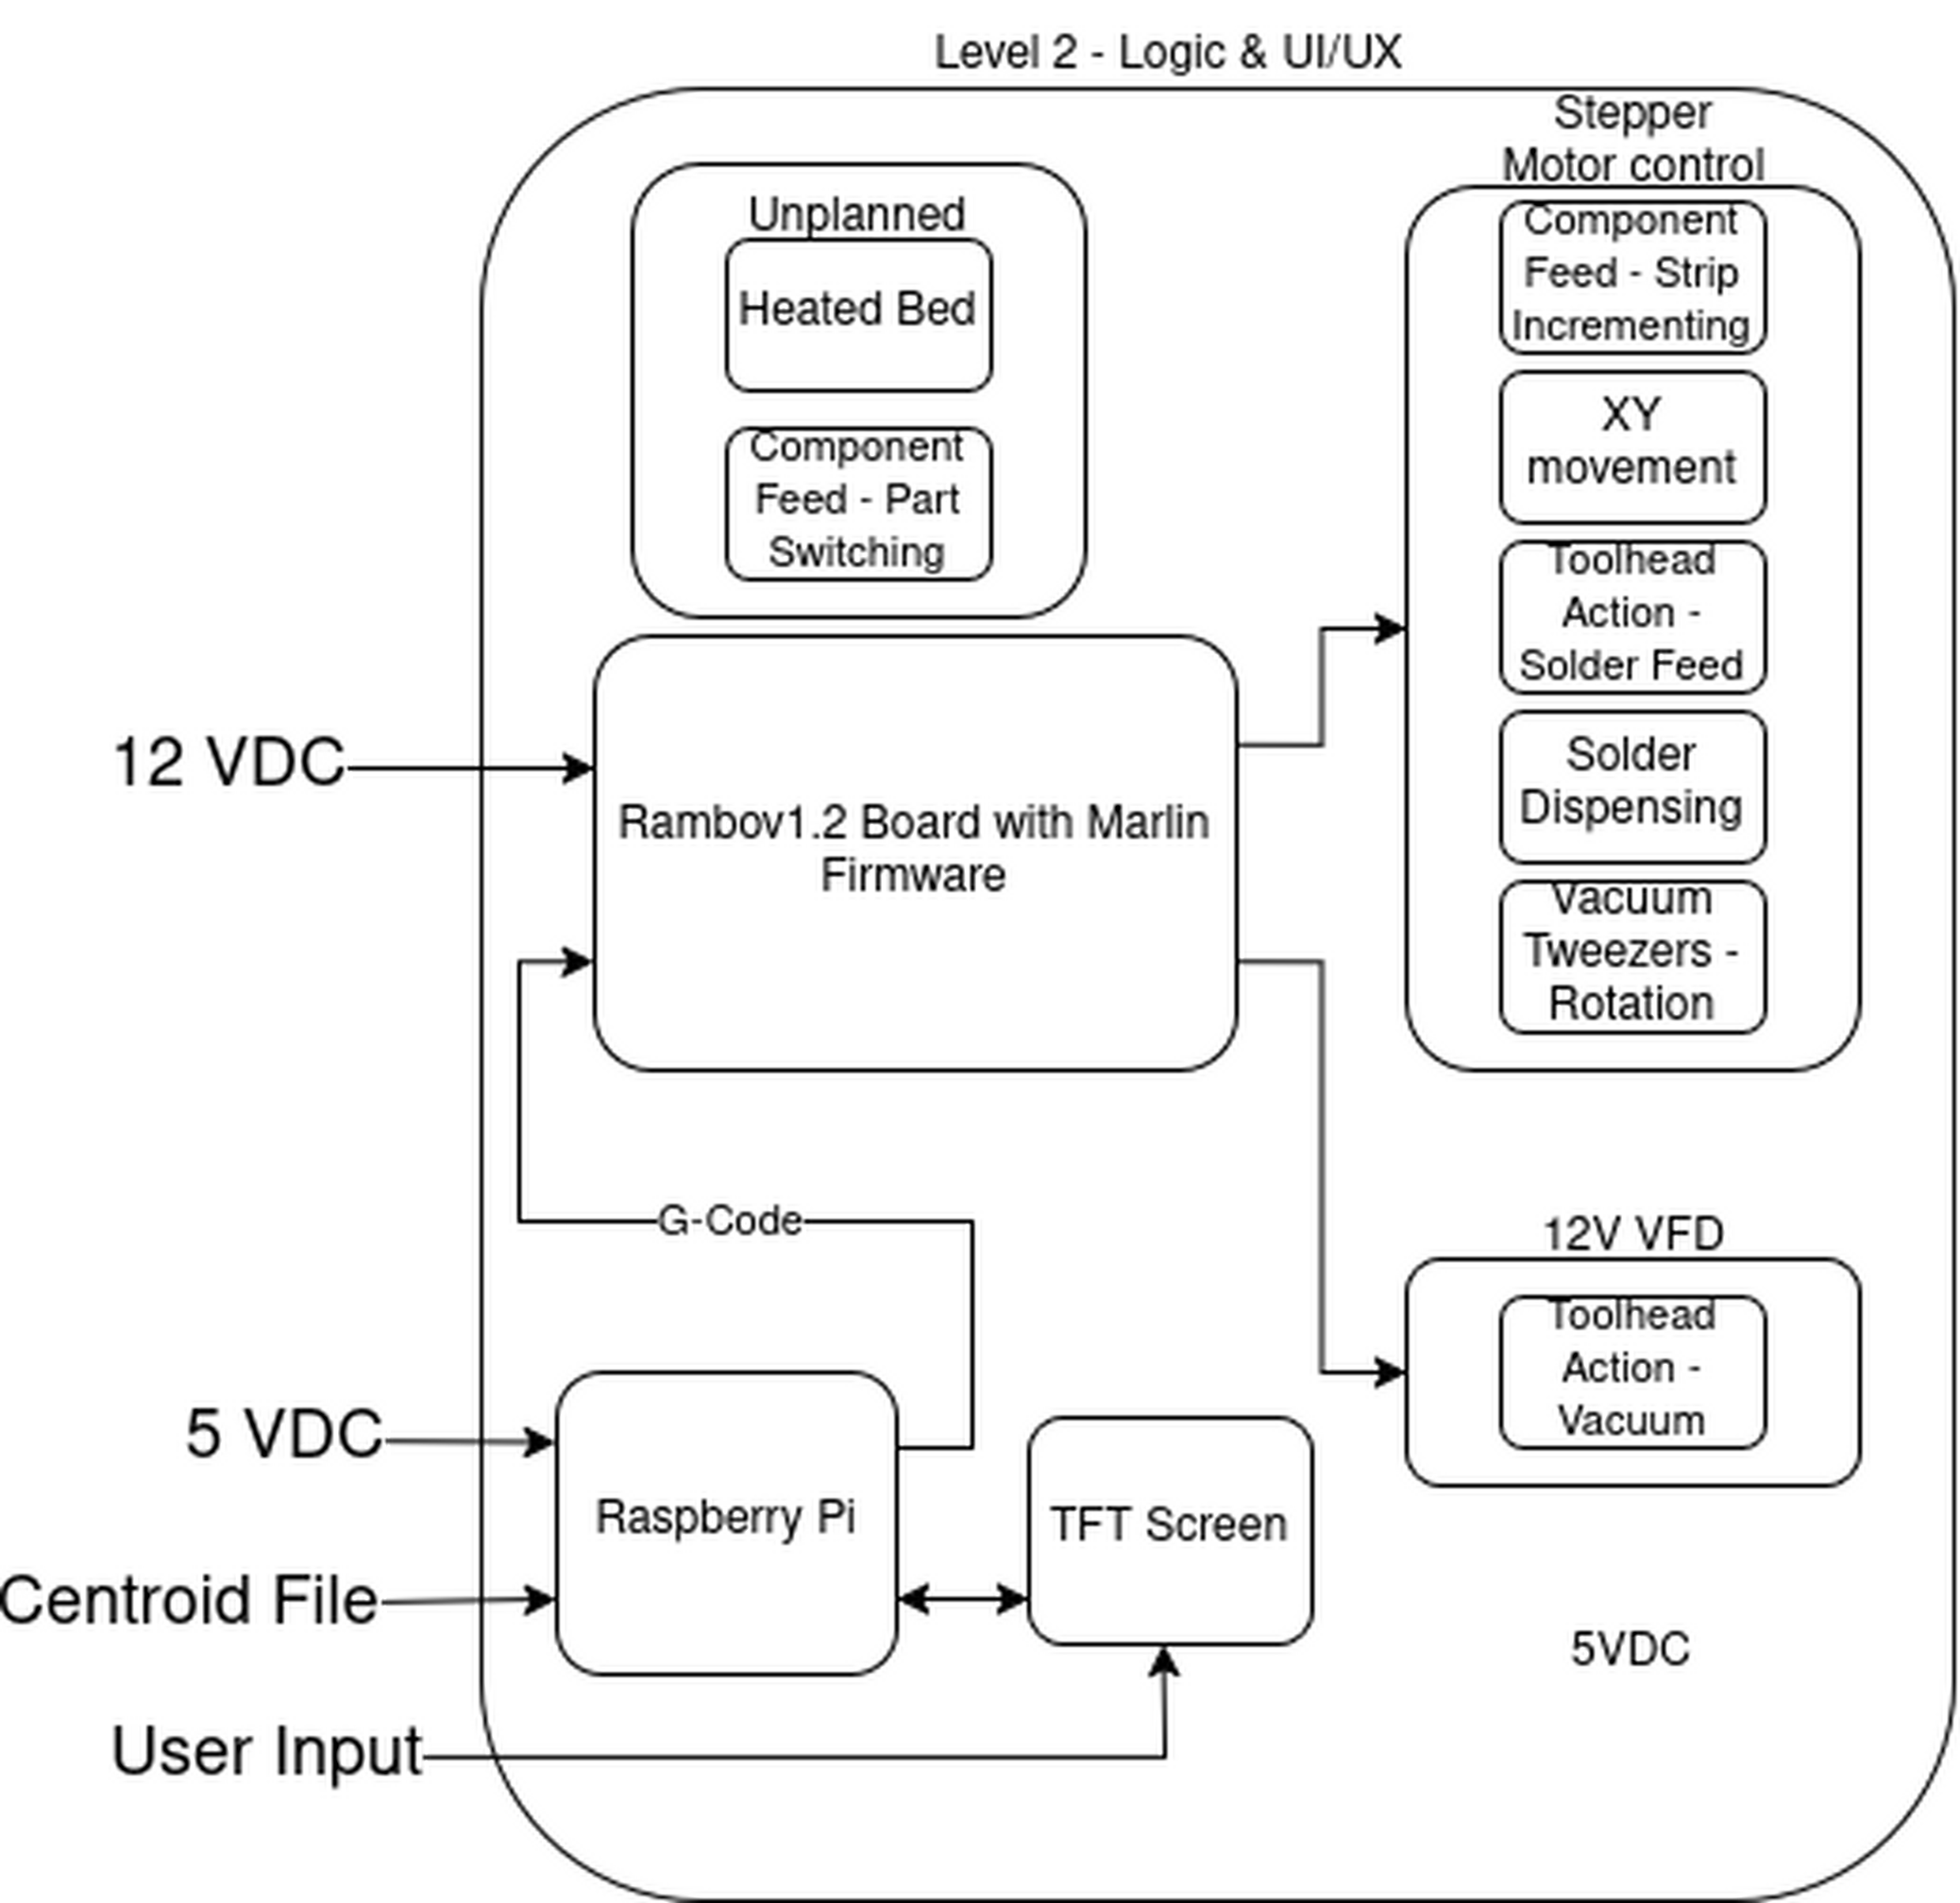
\includegraphics[width=\textwidth]{Level2_logic_ui_ux.png}
\caption{Level 2 Decomposition - Logic and UI/UX}
\label{fig:level2_logic}
\end{figure}

\subsection{Level 2 --- XY Movement}
\begin{figure}[H]
\centering
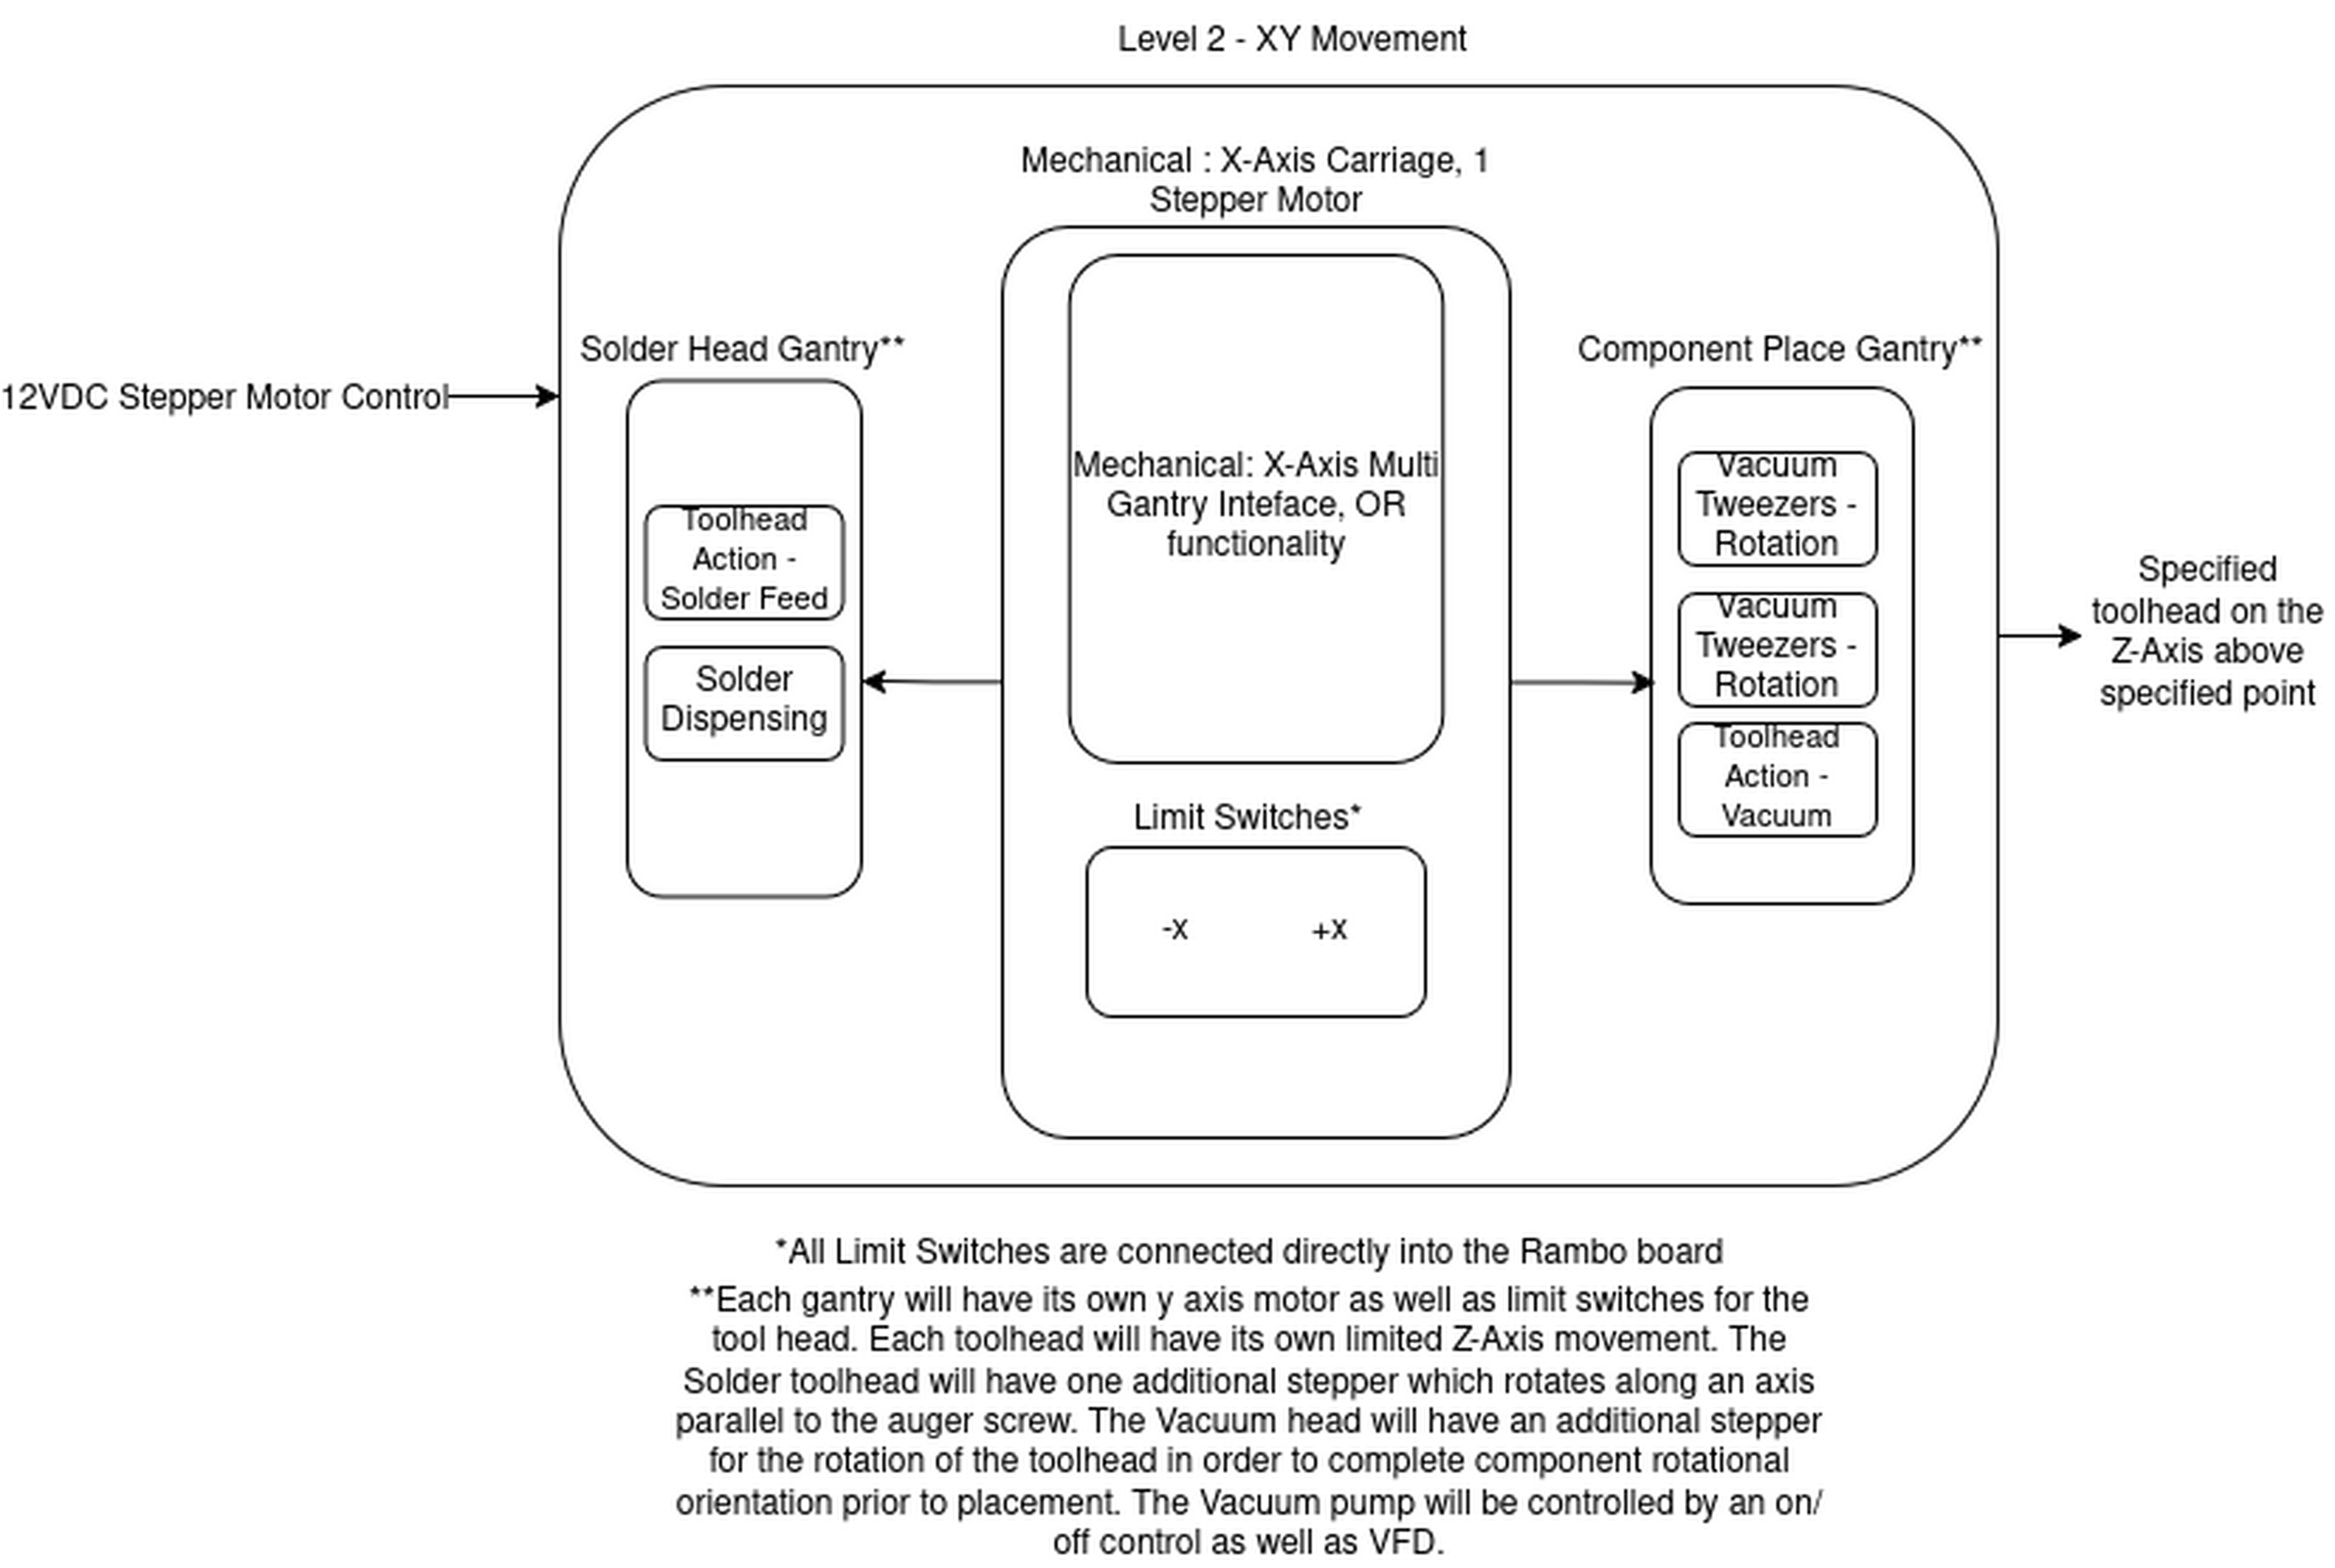
\includegraphics[width=\textwidth]{Level2_xy_movement.png}
\caption{Level 2 Decomposition of the XY Movement}
\label{fig:level2_xy}
\end{figure}


\section{Project Update}
\begin{itemize}
    \item All stepper motors, limit switches, X-Axis Carriage, X-Axis Gantry Interface, Logic Board, and TFT Screen have been sourced.
    \item Placement for Limit Switches, Stepper Motors, Toolheads, and the Unpopulated Board has been planned.
    \item The X-Axis Carriage has been assembled and tested with the Logic Board.
    \item Design for the component feed is underway.
    \item A prototype for centroid file parsing and G-Code translation has been created.
    \item Auger Valve toolhead mechanical and material requirements have been spec'd.
    \item Vacuum head power, control, and mechanical have been spec'd.
    \item The heated bed has not yet entered the planning phase.
\end{itemize} 

\addcontentsline{toc}{section}{References}

\begin{thebibliography}{9}

\bibitem{ul499}
Underwriters Laboratories,
\textit{UL 499: Standard for Electric Heating Appliances},
13th ed., Northbrook, IL: UL LLC, 2014 (with revisions).


\bibitem{ria}
American National Standards Institute / Robotic Industries Association,
\textit{ANSI/RIA R15.06-2012: Industrial Robots and Robot Systems --- Safety Requirements},
Ann Arbor, MI: RIA, 2012.


\bibitem{ipc2581}
IPC,
\textit{IPC-2581 Rev.\ C: Generic Requirements for Printed Board Assembly Products Manufacturing Description Data and Transfer Methodology},
Bannockburn, IL: IPC, 2022.


\bibitem{ul61010}
Underwriters Laboratories,
\textit{UL 61010-1: Safety Requirements for Electrical Equipment for Measurement, Control, and Laboratory Use --- Part 1: General Requirements},
3rd ed., Northbrook, IL: UL LLC, 2012 (with revisions through 2024).


\end{thebibliography}


\end{document}
